\documentclass{beamer}

% Theme settings
\usetheme{Madrid} % Madrid theme provides a similar header and footer structure

% Color definitions (approximate based on the image)
\definecolor{darkblue}{RGB}{40,40,150} % For headers, footers, and boxes
\definecolor{lightblue}{RGB}{180,180,250} % For highlight within boxes
\usepackage[utf8]{inputenc}
\usepackage[T1]{fontenc}
\usepackage[backend=biber,style=numeric]{biblatex}
% Apply colors.sty
\setbeamercolor{palette primary}{bg=darkblue,fg=white}
\setbeamercolor{palette secondary}{bg=darkblue,fg=white}
\setbeamercolor{palette tertiary}{bg=darkblue,fg=white}
\setbeamercolor{palette quaternary}{bg=darkblue,fg=white}
\setbeamercolor{sidebar}{bg=darkblue,fg=white}
\setbeamercolor{frametitle}{bg=darkblue,fg=white}
\setbeamercolor{title}{bg=darkblue,fg=white}
\setbeamercolor{section in head/foot}{bg=darkblue,fg=white}
\setbeamercolor{subsection in head/foot}{bg=darkblue,fg=white}
\setbeamercolor{footline}{bg=darkblue,fg=white}

% For the boxes "Definition", "Theorem", "Example"
\setbeamercolor{block title}{bg=darkblue,fg=white}
\setbeamercolor{block body}{bg=lightblue,fg=black}

% Font settings (default Beamer fonts are often sans-serif, similar to the image)

\usepackage{lmodern} % A good sans-serif font often used with Beamer

% Custom logo (replace 'profmai_logo.png' with your actual logo file)
% Make sure the logo is in the same directory as your .tex file or provide the full path.
\usepackage{tikz}

\addbibresource{bibliography.bib}

\title{Architecture of DeepSeek-V3}
\author{Molnár Botond}
\date{\today} 


\begin{document}


\begin{frame}[noframenumbering]
    \titlepage
\end{frame}

\section{Transformer Models}

\begin{frame}
    \frametitle{Transformer Model Origins}
    Transformer models were first introduced in the Paper "Attention is all you need" in 2017, which arguably launched the artificial intelligence revolution. 
    It introduced the \textbf{self-attention} mechanism which enables the model to understand the whole context of the input without using convolution or sequence based RNNs. \cite{vaswani2017attention}
\end{frame}

\begin{frame}{Why not Convolution?}
    \begin{itemize}
        \item Convolution is excellent at capturing local patterns, but since they have a limited view on the whole context it falls short of capturing global context. \cite{CNNfield}
        \item The weights of CNNs are constant and learned during training, hence applying the same transformation across the same input. (In transformer models these weights come from the self-attention head $\rightarrow$ calculated dynamically)
    \end{itemize}
\end{frame}




\begin{frame}{Why not Recurrent Neural Networks (RNN)?}
    \begin{itemize}
        \item However, the problem of vanishing/exploding gradients has been solved by newer models (LSTM, GRU) they still struggle to maintain "attention". For example, when the model goes through the sequence it might "forget" the early parts of the message or might become insignificant. \cite{heycoachRNN}
        \item Its sequential processing nature prevents efficient parallelization (the $t$-th step depends on the $t-1$-th step), which makes it  time consuming to train the model. \cite{eitcaRNNchallenges}
        \item It has a  fixed sized hidden state (fixed size vector). As the sequence progresses, this vector must continuously update to summarize all relevant past information. For very long sequences, this leads to an information compression problem, where the hidden state cannot retain all the nuances of the entire history. \cite{ibmRNN}
    \end{itemize}
\end{frame}

\begin{frame}{Transformer Model Architecture}
    \begin{center}
        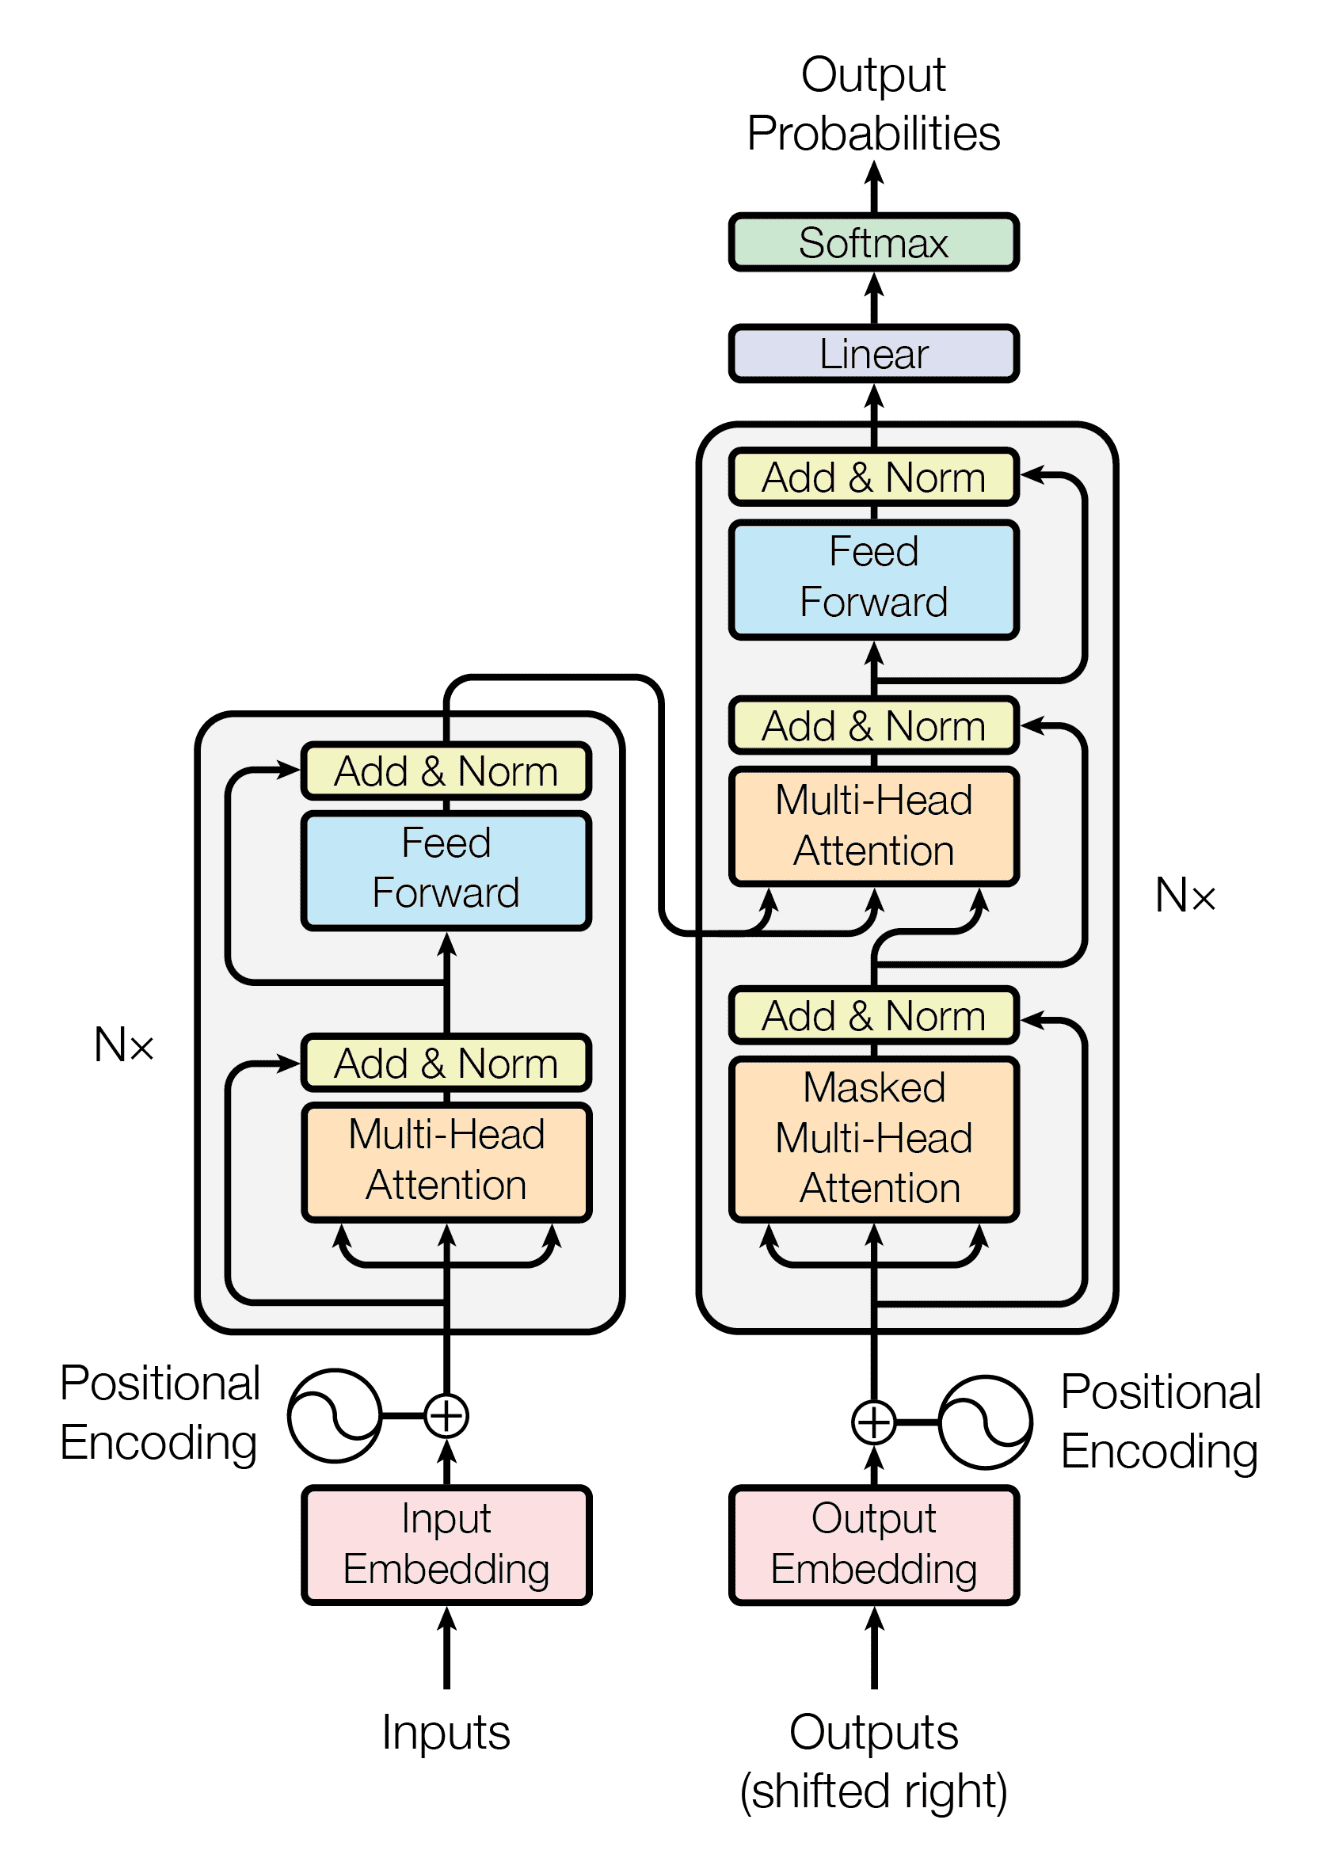
\includegraphics[width=0.4\textwidth]{transformer_model.png}
        \par
        \small Source:  \cite{vaswani2017attention}
    \end{center}
    
\end{frame}

\begin{frame}{Input Processing}
\begin{itemize}
    \item The input text must first be converted into numerical representation, usually using byte-pair encoding done on subword level.
    \item Then each token gets assigned a numerical ID.
\end{itemize}

\textbf{Example:} \\
\vspace{1em}
Raw text: \textit{The quick brown fox jumps.} \\
$\rightarrow$ ["The", "quick", "brown", "fox", "jump", "\#\#s", "."] (\#\# signals the continuation of a word) \\
$\rightarrow$ [101, 234, 567, 890, 123, 456, 789]
\end{frame}


\begin{frame}{Word Embedding}
\begin{itemize}
    \item \textbf{Learned Embeddings}: The transformer uses learned embeddings to convert the input tokens and output tokens to vectors of dimension $d_{model}$. It learns these representation during the training process.
    \item \textbf{Embedding Table}: $V \times d_{model}$ matrix, where each row represents a unique token in the vocabulary
    \item \textbf{Lookup Process}: After the token enters the embedding layer the model simply "looks up" the corresponding row in this embedding table. The entire row is the vector representation for that token.
\end{itemize}


\vspace{1em}
Output:
$$E \in \mathbb{R}^{n \times d_{model}}$$


$V$: vocabulary size \\ $d_{model}$: dimension of the model \\ $n$: number of tokens
    
\end{frame}

\begin{frame}{Position Encoding}
Since transformer models do not have recurrence or convolution, the order of words is not inherently captured, therefore positional encodings must be used. \cite{vaswani2017attention} uses sine and cosine functions to achieve this:

$$ PE_{(\text{pos},2i)} = \sin(\text{pos}/10000^{2i/d_{\text{model}}}) $$
$$ PE_{(\text{pos},2i+1)} = \cos(\text{pos}/10000^{2i/d_{\text{model}}}) $$

$$Input_{model} = E + EP \in \mathbb{R}^{n \times d_{model}}$$

\vspace{1em}
Where $pos$ is the position of the token and $i$ is the dimension.
    
\end{frame}

\section{Encoder Layer}

\begin{frame}{Encoder Attention Head}
    \begin{center}
        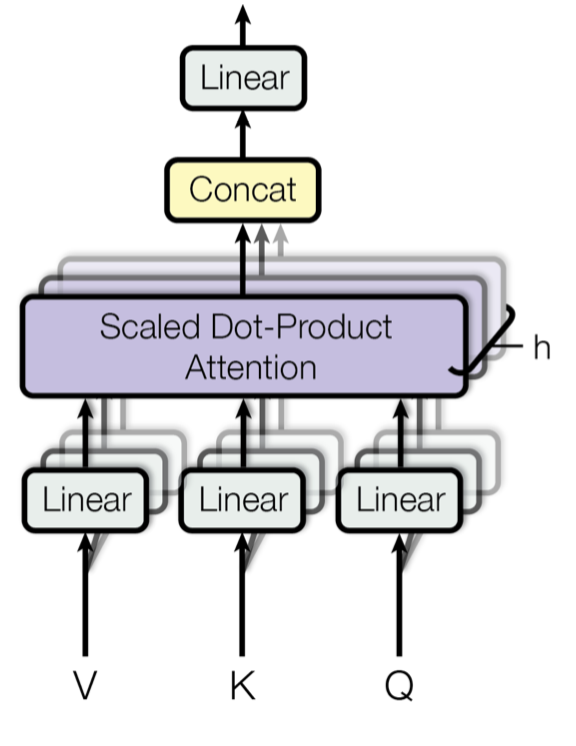
\includegraphics[width=0.4\textwidth]{multi-head-attention_l1A3G7a.png}
        \par
        \small Source:  \cite{vaswani2017attention}
    \end{center}
\end{frame}

\begin{frame}{Encoder Attention Head}

Each encoder attention head's input consists of the $Query$ ($Q$), $Key$ ($K$), $Value$ ($V$).
These values are linearly transformed from the embeddings using learned weights into lower dimensions:

$$Q_i = QW_i^Q$$
$$K_i = KW_i^K$$
$$V_i = VW_i^V$$

Where $Q_i$, $K_i$, $V_i$ $\in \mathbb{R}^{(d_{model}/h)}$, \\
$W_i^Q \in \mathbb{R}^{d_{model} \times d_k}$ \\
$W_i^K \in \mathbb{R}^{d_{model} \times d_k}$ \\
$W_i^V \in \mathbb{R}^{d_{model} \times d_v}$ \\
$h$ is the number of attention heads.  \\
$i$ is the index of the attention head. \cite{vaswani2017attention}
\end{frame}

\begin{frame}{Encoder Attention Head}
\begin{itemize}
    \item \textbf{Query (Q)}: Represents what each token attends to
    \item \textbf{Key (K)}: Represents what each token offers as context
    \item \textbf{Value (V)}: The actual content that gets aggregated
\end{itemize}
\end{frame}

\begin{frame}{Scaled Dot-Product Attention}
    $$ \text{Attention}(Q, K, V) = \text{softmax}\left(\frac{QK^T}{\sqrt{d_k}}\right)V $$

    Where \\ $Q \in \mathbb{R}^{n \times d_k}$, \\
    $K \in \mathbb{R}^{n \times d_k}$, \\
    $V \in \mathbb{R}^{n \times d_v}$. \\
    (In a transformer $d_k = d_v = d_{model}/h$ \cite{vaswani2017attention})

\end{frame}


\begin{frame}{Scaled Dot-Product Attention}
    \begin{itemize}
        \item $QK^T \in \mathbb{R}^{n \times n}$: Similarity between each \textit{Query} and \textit{Key} is computed. Result of the operation is often
        called the \textit{"attention scores"}. A large positive dot product indicates high similarity or 
        relevance between the query at position i and the key at position j. 
        This matrix essentially tells us, for each token in the sequence (represented by a query), how much it relates to every other token in the sequence (represented by keys).
        \item Scaling by $\sqrt{d_k} \left( \frac{QK^T}{\sqrt{d_k}} \right)$: he raw dot products can 
        become very large in magnitude, especially with larger $d_{model}$. 
        This can push the softmax function into regions where its gradients are extremely small (vanishing gradient).
        Dividing by $\sqrt{d_k}$ (the square root of the key dimension) normalizes these dot products, preventing them from becoming too large 
        and ensuring more stable gradients for the softmax.
    \end{itemize}
\end{frame}

\begin{frame}{Scaled Dot-Product Attention}
  \begin{itemize}
    \item Softmax function ($softmax(\cdot)$): The softmax function converts the scores into a probability distribution.
    Let $A_{ij} = \frac{(QK^T)_{ij}}{\sqrt{d_k}}$. Then, the softmax is applied row-wise: $\text{softmax}(A_i) = \frac{e^{A_{i,j}}}{\sum_{k=1}^n e^{A_{i,k}}}$ for each row $i$.
    Output of the $softmax(\cdot)$ is the \textit{"attention weight matrix"}: $W \in \mathbb{R}^{n \times n}$. 
    \item Multiplication with the \textit{Value (V)} matrix ($W \cdot V$): This multiplication effectively takes a weighted sum of the \textit{Value} vectors, 
    where the weights are given by the attention weight matrix $W$. This step aggregates the information from the relevant parts of the sequence into a single context-aware representation for each position.
    $$head_j = W \cdot V$$
    $$head_j \in \mathbb{R}^{n \times d_v}$$
    Where $j$ is the index of the attention head.
  \end{itemize}
\end{frame}


\begin{frame}{Concatenate Outputs From Attention Heads}

$$MultiHead(Q,K,V) = Concat(head_1, ..., head_h)W^O \in \mathbb{R}^{n \times d_{model}}$$

where $head_j = Attention(QW_i^Q, KW_i^K, VW_i^Q) \in \mathbb{R}^{n \times (h \cdot d_k)}$, \\ 
(since $h \cdot d_k = h \cdot (d_{model}/h) = d_{model}$) \\
$W^O \in \mathbb{R}^{hd_v \times d_{model}}$ : Learned linear projection\\
$n$: sequence length

\end{frame}

\begin{frame}{Add and Norm Layer}
  The output of the Multi-Head Attention is added to its input ($Z^{(l-1)}$) and then layer normalized.

  $$ Z_{attention\_normalized} = LayerNorm(Z^{(l-1)} + MultiHead(\cdot)) \in \mathbb{R}^{n \times d_{model}} $$
\end{frame}


\begin{frame}{Layer Normalization}
  For an input vector $x$ (a row in the matrix), it normalizes over the features \cite{ba2016layer}:
  $$ \mu = \frac{1}{d_{\text{model}}} \sum_{i=1}^{d_{\text{model}}} x_i \text{ (mean)} $$
  $$ \sigma^2 = \frac{1}{d_{\text{model}}} \sum_{i=1}^{d_{\text{model}}} (x_i - \mu)^2 \text{ (variance)} $$
  $$ \text{LayerNorm}(x_i) = \gamma \frac{x_i - \mu}{\sqrt{\sigma^2 + \epsilon}} + \beta $$
   $\gamma$ and $\beta$ are learned scaling and shifting parameters, respectively. \\
   $\epsilon$ is a small constant for numerical stability (to prevent division by zero).
\end{frame}


\begin{frame}{Position-wise Feed-Forward Network}
  This sub-layer is applied to each position independently and identically. 
  It consists of two linear transformations with a ReLU activation in between. \\
  Let the input be $Z_{attention\_normalized}$

  $$ \text{FFN}(Z_{attention\_normalized}) = \max(0, xW_1 + b_1)W_2 + b_2 $$

  \begin{itemize}
    \item $ W_1 \in \mathbb{R}^{d_{\text{model}} \times d_{\text{ff}}} \text{ (e.g., } 512 \times 2048) $
    \item $b_1 \in \mathbb{R}^{d_{ff}}$
    \item $max(0, \cdot)$ is the ReLU activation function
    \item $W_2 \in \mathbb{R}^{d_{\text{ff}} \times d_{\text{model}}} \text{ (e.g., } 2048 \times 512)$
    \item $b_2 \in \mathbb{R}^{d_{\text{model}}}$
    \item Let the output be $FFN_{output} \in \mathbb{R}^{n \times d_{model}}$ $\rightarrow$ This will be passed to another \textbf{Add and Norm} sublayer
    whose output will be passed to the next encoder layer. 
  \end{itemize}
\end{frame}


\begin{frame}{Final Encoder Output}
  After passing through all $N$ encoder layers, the output of the last layer ($Z^{(N)}$) is a sequence of $n$ vectors, each of dimension $d_{\text{model}}$. These vectors are dense, contextualized representations of the input sequence. This final output of the 
  encoder stack is then passed to the decoder's "encoder-decoder attention" mechanism. \cite{vaswani2017attention}
\end{frame}

\section{Decoder Layers}

\begin{frame}{Decoder Layer}
  The decoder in the Transformer model is responsible for generating the output sequence one token at a time, incorporating context from both the input sequence (via the encoder)
  and the tokens it has already generated. It operates in an auto-regressive fashion.
  
  Each of the N identical layers within the decoder stack is composed of three 
  main sub-layers, each followed by a residual connection and layer normalization.

  The main difference to the encoder layer is a new sub-layer, the multi-head self-attention.
\end{frame}

\begin{frame}{Decoder Layer}
  \begin{itemize}
    \item Let the input be $Y^{(l-1)}$ for the current decoder layer $l$. (output from the previous decoder layer 
    or the combined embedding and positional encoding of the partial output sequence for the first layer)
    \item The encoder's final output $ Z_{\text{enc}}^{(N)} $ , serves as the memory for the encoder-decoder attention.
  \end{itemize}

  \begin{itemize}
    \item $Y^{(l-1)} \in \mathbb{R}^{m \times d_{model}}$ 
    \item $m$: current length of the partial output sequence being generated
    \item $ Z_{\text{enc}}^{(N)} \in \mathbb{R}^{n \times d_{\text{model}}} $
  \end{itemize}
  
\end{frame}

\begin{frame}{Masked Multi-Head Self-Attention Sub-layer}
  \textbf{1. Input Projections for Q, K, V:}
  \begin{itemize}
    \item The input to this sub-layer is $Y^{(l-1)}$.
    \item For each of the $h$ attention heads ($j = 1, \dots, h$), $Y^{(l-1)}$ is linearly projected into Query ($Q_j$), Key ($K_j$), and Value ($V_j$) matrices using learned weight matrices $W^Q_j, W^K_j, W^V_j \in \mathbb{R}^{d_{\text{model}} \times d_k}$ (where $d_k = d_v = d_{\text{model}}/h$).
    \item $ Q_j = Y^{(l-1)}W^Q_j $
    \item $ K_j = Y^{(l-1)}W^K_j $
    \item $ V_j = Y^{(l-1)}W^V_j $
    \item $Q_j, K_j, V_j \in \mathbb{R}^{m \times d_k}$.
  \end{itemize}
\end{frame}

\begin{frame}{Masked Attention}
  \textbf{2. Masked Scaled Dot-Product Attention:}
  \begin{itemize}
      \item The core attention calculation is performed:
      $$ \text{head}_j = \text{softmax}\left(\frac{Q_j K_j^T + \text{Mask}}{\sqrt{d_k}}\right)V_j $$
      \item \textbf{The crucial difference here is the "Mask."} This is a look-ahead mask (upper triangular matrix of negative infinities) that is applied to the attention scores before the softmax function.
      \item It prevents each position in the decoder from attending to subsequent positions. When predicting the $i$-th token, the mask ensures that the calculation for $\text{head}_j$ only considers information from tokens at positions $1, \dots, i-1$. This is essential for maintaining the 
      auto-regressive property of the decoder, ensuring that predictions for future tokens do not influence current token generation.
      \item Everithing else works the same as in the encoder layers.
      \item Output: $\text{head}_j \in \mathbb{R}^{m \times d_k}$.
      \item $Mask \in \mathbb{R}^{m \times m}$
  \end{itemize}
\end{frame}


\begin{frame}{Decoder Multi-Head Attention}
  Acts as the bridge between the input sequence 
  (processed by the encoder) and the output sequence (being generated by the decoder). \\
  Inputs:
  \begin{itemize}
    \item $K_{\text{enc}} = \text{Encoder Output}$
    \item $V_{\text{enc}} = \text{Encoder Output}$
    \item $Q_{\text{dec}} = \text{Output of decoder's masked self-attention layer}$
  \end{itemize}
\end{frame}


\begin{frame}{Encoder-Decoder Attention: Core Mechanism}
    \begin{itemize}
        \item Now, the $Q_{\text{dec}}$ (the decoder's current understanding of the partial output) is used to \textbf{query} the $K_{\text{enc}}$ (the encoder's representation of the entire input).
        \item The attention mechanism calculates compatibility scores between each part of the decoder's query and all parts of the encoder's keys.
        \item This determines which parts of the input sentence are most relevant to predicting the \textit{next} token in the output sequence.
    \end{itemize}
\end{frame}

\begin{frame}{Encoder-Decoder Attention: Formula}
    Mathematically, for each attention head $j$ in the encoder-decoder attention:
    $$ \text{head}_j = \text{softmax}\left(\frac{Q_{\text{dec},j}K_{\text{enc},j}^T}{\sqrt{d_k}}\right)V_{\text{enc},j} $$
    This formula is similar to the self-attention formula, but uses different sources for $Q$, $K$, and $V$.

    \begin{itemize}
      \item $Q_{dec, j} \in \mathbb{R}^{n \times d_k}$: Query from the masked multi-head self-attention sub-layer.
      \item $K_{enc, j} \in \mathbb{R}^{n \times d_k}$: Key 
      \item $V_{enc, j} \in \mathbb{R}^{n \times d_v}$
      \item $head_j \in \mathbb{R}^{m \times d_v}$
    \end{itemize}
\end{frame}

\begin{frame}{Token Prediction}
  After the input went through all the decoder layers, the output takes the hidden vector ($h_{last} \in \mathbb{R}^{d_{model}}$ the next generated token's representation) applies a linear layer
  which projects $h_{last}$ into the a vector of the vocabulary's space $V_{vocab}$. Afterwards the model runs $softmax$ on this
  result which will transform the vector into a probability distribution.

  Input:
  \begin{itemize}
    \item $Y^{(N)}_{dec} \in \mathbb{R}^{m \times d_{model}}$: Output of the last encoder layer.
  \end{itemize}
\end{frame}

\begin{frame}{Linear Layer}
  $$Logits = h_{last}W_{out}+b_{out}$$

  \begin{itemize}
    \item $W_{out} \in \mathbb{R}^{d_{model} \times V_{vocab}}$: Learned weight matric for the output linear layer.
    \item $b_{out} \in \mathbb{R}^{V_{vocab}}$: This is the learned bias vector for the output linear layer.
    \item $Logits \in \mathbb{R}^{V_{vocab}}$: The resulting vector. Each element in this vector is a raw, unnormalized score (a "logit") corresponding to a specific token in the vocabulary.
  \end{itemize}
\end{frame}

\begin{frame}{Vocabulary Probability Distribution}
  The \textit{Logits} vector represents a raw likelihood values, to acquire the probabilities of these
  tokens we apply softmax function on the vector, which gives the probability of each token in the vocabulary.

  $$P = Softmax(Logits) \in \mathbb{R}^{V_{vocab}}$$

\end{frame}

\begin{frame}{Token Selection}
  Multiple strategies for choosing the next token:
  \begin{itemize}
    \item \textbf{Greedy Decoding}:  The simplest method, where the token with the absolute highest probability
     is always chosen. This is deterministic but can sometimes lead to sub-optimal or repetitive sequences.
     \item \textbf{Beam Search}: A more sophisticated method that explores multiple promising sequences simultaneously. It keeps track of the 'k' most probable partial sequences (the "beam") at each step and extends them, 
     ultimately selecting the most probable complete sequence.\cite{analyticsvidhya_beam_search}
     \item \textbf{Sampling (e.g., Top-K, Nucleus Sampling)}: Instead of always picking the highest probability token, these methods introduce an element of randomness.
        \begin{itemize}
            \item \textbf{Top-K Sampling} involves randomly sampling from only the 'k' most probable tokens.
            \item \textbf{Nucleus Sampling (Top-P Sampling)} samples from the smallest set of tokens whose cumulative probability exceeds a predefined threshold 'p'. These methods help generate more diverse and less predictable outputs, which can be desirable for creative tasks.
        \end{itemize}
  \end{itemize}
\end{frame}

\begin{frame}{Problems with Traditional Transformer Architecture}
  Problems with regular transformer LLMs include \cite{shazeer2017outrageously} \cite{dai2024deepseekmoe}:
  \begin{itemize}
    \item \textbf{Limited Scalability of Total Parameters}: To increase the model's capacity the
    traditional way is to increase the number of parameters in the model.
    \item \textbf{Proportional Computational Cost Increate with Parameter Count}: The computational costs
    linearly increase with the parameter count, making scaling up very expensive and computationally prohibitive beyond a certain point.
    \item \textbf{Less Efficient Parameter Utilization and Specialization}: In a dense Transformer, every parameter in every FFN layer processes every token. 
    This means the network has to find a "one-size-fits-all" set of parameters for all inputs. This can lead to redundancy or inefficiency.
  \end{itemize}
\end{frame}

\begin{frame}{Mixture of Experts Architecture}
  \begin{center}
        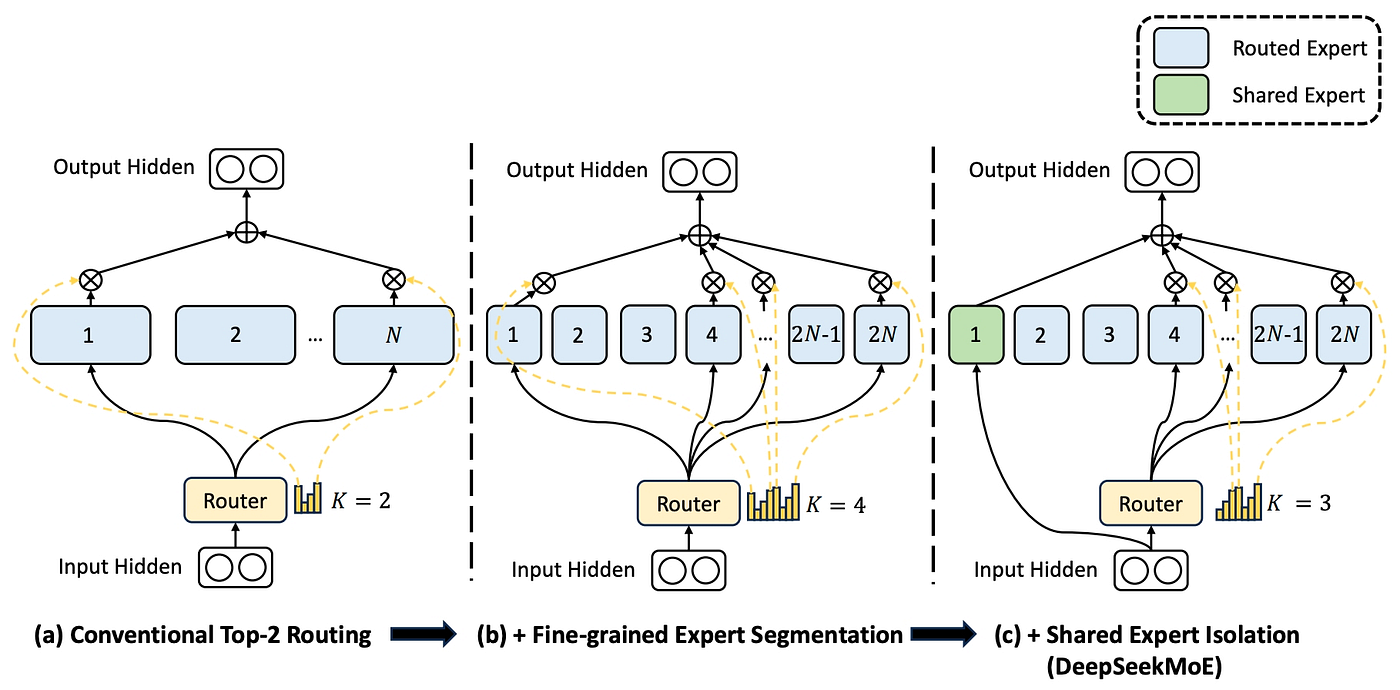
\includegraphics[width=0.9\textwidth]{Moe.png}
        \par
        \small Source:  \cite{dai2024deepseekmoe}
    \end{center}
\end{frame}

\begin{frame}{Mixture of Experts Architecture}
  \begin{itemize}
        \item \textbf{A Router (Gating Network)}: This small neural network takes the token's representation and determines which experts are most relevant for processing it.
        \item \textbf{A Pool of Experts}: These are typically individual FFNs, each specializing in different aspects of the input.
        \item \textbf{Sparse Activation}: Instead of activating all experts, the router selects and activates only a small subset (e.g., top-K) of experts for each token. Their outputs are then combined, usually as a weighted sum based on the router's scores.
    \end{itemize}
    \cite{shazeer2017outrageously}

    $$ y = \sum_{i=1}^{n} G(x)_i E_i(x) $$
\end{frame}

\begin{frame}[allowframebreaks]{Mixture of Experts Architecture}

  $$ \mathbf{h}^l_t = \sum_{i=1}^{N} \left(g_{i,t} \text{FFN}_i (\mathbf{u}^l_t)\right) + \mathbf{u}^l_t $$
  $$ g_{i,t} = \begin{cases} s_{i,t}, & s_{i,t} \in \text{Topk}(\{s_{j,t}|1 \le j \le N\}, K), \\ 0, & \text{otherwise}, \end{cases} $$
  $$ s_{i,t} = \text{Softmax}_i \left(\mathbf{u}_t^T \mathbf{e}_i^l\right), $$
  

  \begin{itemize}
    \item $N$: Total number of experts
    \item $FFN_i(\cdot)$: $i$-th expert FFN
    \item $g_{i,t}$: Gate value for the $i$-th expert
    \item $s_{i,t}$: Token-to-expert affinity
    \item $TopK(\cdot, K)$: set
    comprising $K$ highest affinity scores among those calculated for 
    the $t$-th token and all $N$ experts.
    \item $\mathbf{h}^l_t$: Output hidden state
    \item $\mathbf{u}^l_{1:T} \in \mathbb{R}^{T \times d_{model}}$: hidden states of all tokens after
    the $l$-th attention module
    \item $\mathbf{e}_i^l \in \mathbb{R}^{d_{model}}$ 
  \end{itemize}
  \cite{dai2024deepseekmoe}
\end{frame}




\begin{frame}{DeepSeek-V3's MoE Architecture}
  Core innovations in DeepSeek's MoE architecture \cite{dai2024deepseekmoe}:
  \begin{itemize}
    \item \textbf{Fine-Grained Expert Segmentation}: DeepSeek segments each conceptual "expert FFN" into m smaller, distinct experts. 
    This is achieved by reducing the intermediate hidden dimension of each expert's FFN to $1/m$ times its original size.
    \item \textbf{Shared Experts}: DeepSeek introduces a fixed number of "shared experts" that are always active.
    \item \textbf{Auxiliary-Loss-Free Load Balancing}: DeepSeek's router design and routing algorithm are inherently constructed to promote balanced expert 
    utilization without needing a separate auxiliary loss term during training. This simplifies the training objective and can lead to more robust balance.
  \end{itemize}
\end{frame}


\begin{frame}{Shared Experts}
  
  \textbf{Problem}: In a purely sparse MoE, all experts are specialized. However, much of the knowledge required by an LLM is universal (e.g., basic grammar, common facts). 
  Forcing specialized experts to repeatedly learn this common knowledge is redundant. \cite{dai2024deepseekmoe}


  The shared expert mechanism solves knowledge redundancy between experts, meaning an expers more diverse 
  more in depth knowledge, since the shared expert takes care of common knowledge. \cite{dai2024deepseekmoe}
\end{frame}

\begin{frame}{Shared Experts}
\textbf{Mechanism}:
\begin{enumerate}
  \item \textbf{Always-On Activation}: For every token processed by an MoE layer, its representation is simultaneously sent to:
    \begin{itemize}
      \item The router, which then selects a subset of "routed experts."
      \item All of the pre-designated shared experts.
    \end{itemize} 
  \item \textbf{Output Integration}: The output of the shared experts is directly added to the weighted sum of the outputs from the selected routed experts. They do not have a gating coefficient applied to their 
  output (or effectively have a fixed coefficient of 1), as they are universally important.
\end{enumerate}  
\end{frame}

\begin{frame}{Shared Experts}
  $$ \mathbf{h}^l_t = \sum_{i=1}^{K_s} \text{FFN}_i (\mathbf{u}^l_t) + \sum_{i=K_s+1}^{mN} \left(g_{i,t} \text{FFN}_i (\mathbf{u}^l_t)\right) + \mathbf{u}^l_t $$
  $$ g_{i,t} = \begin{cases} s_{i,t}, & s_{i,t} \in \text{Topk}(\{s_{j,t}|K_s + 1 \le j \le mN\}, mK - K_s), \\ 0, & \text{otherwise}, \end{cases} $$
  $$ s_{i,t} = \text{Softmax}_i \left(\mathbf{u}_t^T \mathbf{e}_i^l\right). $$

  \begin{itemize}
    \item $K_s$: Number of shared experts
    \item $m$: Number of fine-grained experts (later)
  \end{itemize}
  \cite{dai2024deepseekmoe}
\end{frame}

\begin{frame}{Shared Experts Benefits Compared to Treaditional Method}
  \begin{itemize}
    \item \textbf{Deeper Specialization for Routed Experts}: By offloading universal knowledge to shared experts, the vast pool of fine-grained, 
    routed experts can truly focus on highly specific, nuanced, or conditional patterns.
    \item \textbf{Enhanced Model Robustness}: Shared experts ensure that fundamental capabilities 
    and common knowledge are always present and contribute to the model's output. This makes the model more reliable and robust, especially 
    when dealing with inputs that might not perfectly align with any specific niche expert.
    \item \textbf{Improved Generalization}: By consolidating general knowledge, the model can 
    generalize better to unseen data, as the core understanding is consistently applied.
    \cite{dai2024deepseekmoe}
  \end{itemize}
\end{frame}


\begin{frame}{Fine-Grained Expert Segmentation}
  \textbf{Problem}:  
  \begin{itemize}
    \item \textbf{Coarse Granularity of Expertise}: A large FFN expert might still learn a broad range of knowledge, 
    leading to overlap or redundancy if different experts acquire similar functionalities.
    \item \textbf{Limited Combinatorial Flexibility}: If you have $N$ experts and select $K$ of them, the number of unique combinations, 
    while large, is constrained by the size of the individual experts. 
    Finer distinctions in expertise are often desirable for complex tasks.
  \end{itemize}

  \cite{dai2024deepseekmoe}
\end{frame}

\begin{frame}{Fine-Grained Expert Segmentation}
  $$ \mathbf{h}^l_t = \sum_{i=1}^{mN} \left(g_{i,t} \text{FFN}_i (\mathbf{u}^l_t)\right) + \mathbf{u}^l_t $$
    $$ g_{i,t} = \begin{cases} s_{i,t}, & s_{i,t} \in \text{Topk}(\{s_{j,t}|1 \le j \le mN\}, mK), \\ 0, & \text{otherwise}, \end{cases} $$
    $$ s_{i,t} = \text{Softmax}_i \left(\mathbf{u}_t^T \mathbf{e}_i^l\right) $$
\end{frame}

\begin{frame}{Fine-Grained Expert Segmentation}
  \textbf{Mechanism}:
  \begin{itemize}
    \item \textbf{Segmentation Factor ($m$)}: A chosen factor (e.g., m=4) by which the FFN's 
    intermediate hidden dimension is divided. 
    \item \textbf{Creating "Smaller Experts"}: If a conceptual "parent" FFN expert would have had a hidden dimension of $D_{\text{hidden\_original}}$, then DeepSeek effectively segments it into $m$ "fine-grained experts," 
    each of which has an intermediate hidden dimension of $D_{\text{hidden\_original}}/m$.
    \item \textbf{Total Expert Pool}: If the model conceptually starts with $N$ experts, this segmentation process means 
    the actual pool of distinct, routable experts becomes $N \times M$ fine-grained experts.
  \end{itemize}
\end{frame}

\begin{frame}[allowframebreaks]{Fine-Grained Expert Segmentation}
  \begin{enumerate}
    \item \textbf{First Linear Layer + Activation}:
      $$ \mathbf{h}_j = \text{Activation}(\mathbf{x}W_{1,j} + \mathbf{b}_{1,j}) $$
      \begin{itemize}
          \item $\mathbf{x} \in \mathbb{R}^{D_{\text{model}}}$ is the input token representation.
          \item $W_{1,j} \in \mathbb{R}^{D_{\text{model}} \times (D_{\text{hidden\_original}}/m)}$ is the weight matrix for the first linear transformation.
          \item $\mathbf{b}_{1,j} \in \mathbb{R}^{(D_{\text{hidden\_original}}/m)}$ is the bias vector.
          \item $\mathbf{h}_j \in \mathbb{R}^{(D_{\text{hidden\_original}}/m)}$ is the intermediate hidden state for this specific fine-grained expert.
      \end{itemize}
    \item \textbf{Second Linear Layer}:
      $$ \mathbf{y}_j = \mathbf{h}_j W_{2,j} + \mathbf{b}_{2,j} $$
      \begin{itemize}
          \item $W_{2,j} \in \mathbb{R}^{(D_{\text{hidden\_original}}/m) \times D_{\text{model}}}$ is the weight matrix for the second linear transformation.
          \item $\mathbf{b}_{2,j} \in \mathbb{R}^{D_{\text{model}}}$ is the bias vector.
          \item $\mathbf{y}_j \in \mathbb{R}^{D_{\text{model}}}$ is the output contribution of this fine-grained expert.
      \end{itemize}
    \item \textbf{Gating Coeficient}: The output of each expert then multiplied by the gating coef $g_{j,t}$.
    $$  $$
  \end{enumerate}
\end{frame}

\begin{frame}{Fine-Grained Expert Segmentation Benefits}
  \begin{itemize}
    \item \textbf{Increase in Combinatorial Flexibility}: Allows the model to learn highly custized groups of expertise.
    \item \textbf{Enhanced and Deeper Specialization}: Since each fine-grained expert is smaller it is naturally pushed to specialize 
    in a much narrower and more specific aspect of knowledge or transformation.
    \item \textbf{Reduced Redundancy Across Experts}: More efficient utilization of the model's vast parameter count.
    \item \textbf{Effective Scaling to Unprecedented Sizes}: This mechanism is crucial for enabling the creation of models with hundreds of billions or even trillions of parameters. It allows the model to absorb and organize an immense amount of information by segmenting it into manageable, 
    highly specialized chunks, which can then be sparsely activated.
  \end{itemize}
  \cite{dai2024deepseekmoe} \cite{gopubby_deepseekv3}
\end{frame}


\begin{frame}{Is there truly an improvement?}
  The authors measured specialization by disabling the top routed experts, since experts should be less
  replaceble when they are more specialized $\rightarrow$ disabling the top routed expert should impact a bigger
  impact on performance.

  They disabled top routed experts in both DeepSeekMoE and GShard x 1.5 (serving as baseline) and looked at the 
  Pile loss at each number of disabled experts and the results suggested that disabling experts has a bigger
  effect on DeepSeek than on Gshard therefore DeepSeeekMoE is more specialized. \cite{dai2024deepseekmoe} \cite{gopubby_deepseekv3}
  
\end{frame}


\begin{frame}
  \begin{center}
        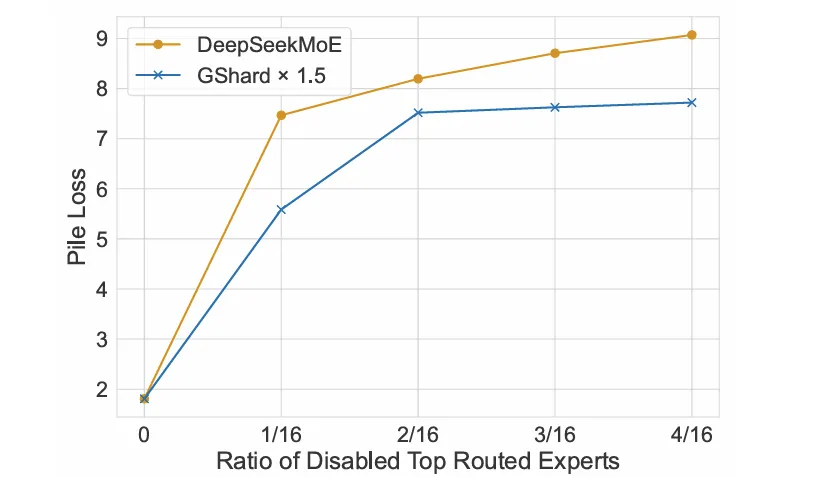
\includegraphics[width=0.9\textwidth]{pile.png}
        \par
        \small Source:  \cite{dai2024deepseekmoe}
    \end{center}
\end{frame}


\begin{frame}[allowframebreaks]
    \frametitle{References}
    \printbibliography
\end{frame}

\end{document}